\documentclass[tikz,border=10pt]{standalone}
\usepackage{tikz}
\usetikzlibrary{calc, angles, decorations.markings}
\usepackage{sgeometry} 
\tikzset{test/.style={line width=0.8pt, red}}

\begin{document}
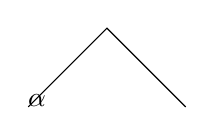
\begin{tikzpicture}
  \coordinate (a) at (0,0);
  \coordinate (b) at (1,1);
  \coordinate (c) at (2,0);
  \draw (a) -- (b) -- (c);
  \Angle[label=$\alpha$, count=3, offset=0.05cm, shift={0,-1.2}, style=test]{a}{b}{c}
\end{tikzpicture}

\begin{tikzpicture}
  \coordinate (A) at (0,0);
  \coordinate (B) at (3,1);
  \coordinate (C) at (1,3);
  \coordinate (D) at (5,3);
  \coordinate (E) at (6,0);
  \coordinate (F) at (4,-1);

  \draw (a) -- (b) -- (c) -- (d) -- (e) -- cycle;

  \MarkSide{a}{b}
  \MarkSide[shape=double line, style=blue]{b}{c}
  \MarkSide[shape=triple line, style=red]{c}{d}
  \MarkSide[shape=vee, style=green!70!black]{d}{e}
  \MarkSide[shape=wave, style=orange]{e}{a}
\end{tikzpicture}

\begin{tikzpicture}
  \coordinate (a) at (3,0);
  \coordinate (b) at (-1,0);
  \coordinate (c) at (-1,4);
  \draw (a) -- (b) -- (c);
  \RightAngle[style=red]{a}{b}{c}
\end{tikzpicture}

\end{document}
